%!TEX root = cscw2019-comic.tex
\section{Appendix}
\label{sec:Appendix}
% \section{Model Criticism}
\subsection{Posterior Predictive Check}
\label{sub:Posterior Predictive Check}

In this section, we examine how well our model makes predicts the observed data.

\begin{figure*}[htb]
    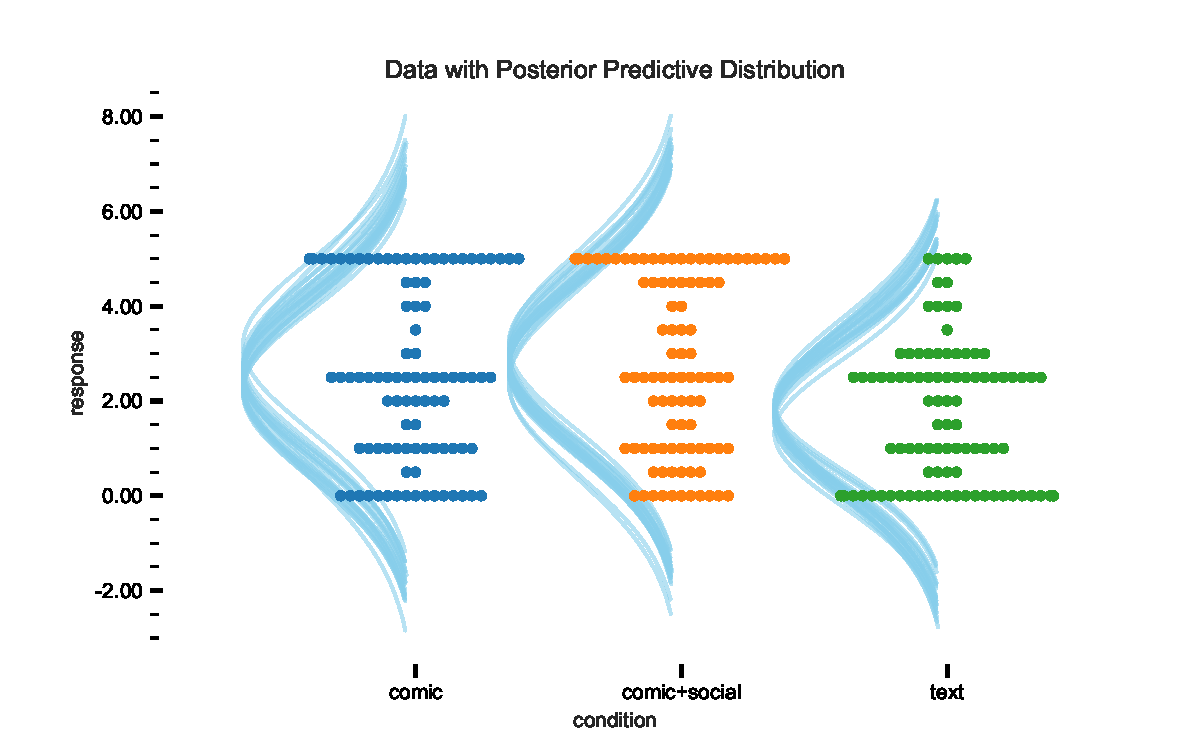
\includegraphics[width=1\textwidth]{./figures/posterior_predictions.pdf}
    \caption{Posterior prediction check: traces from the posterior distributions for each condition are super-imposed onto the observational data. The $x$-axis shows the three conditions, while the $y$-axis shows the contribution (each dot corresponds to a response by a single subject). The $t$-distribution captures the heavy tails, and we also see that the scale of the $t$-distribution in the case of the text condition is smaller than the other two cases. }
    \label{fig:posteriorprediction}
\end{figure*}

One of the advantages of a Bayesian model is that one can use the model to make predictions. Since the probabilistic model is generative, we can simply draw observations from the model. When we superimpose the posterior distribution traces onto the observational data in~\Cref{fig:posteriorprediction} we can observe three things. First, notice that the mean contribution for the `text' condition is less than the `comic' or the `comic+social norm' conditions, which seems reasonable given the increased number of \$0.0 contributions for the `text' condition in comparison to the other two cases. Second, the use of the heavy-tailed $t$-distribution captures well the tails of the distribution at \$0 and at \$5.0. Third, the scale of the distribution for the text condition is smaller than the scales for the two comic conditions, justifying our use of different scale parameters $\sigma_j$ for the three experimental conditions.


Having discussed posterior-prediction checks, next, we discuss alternatives to the model.


\subsection{Alternative Models}
\label{sub:Alternative Models}

As a first instance, consider a similar model, except that the scale parameter of the likelihood function is \textit{not nested} like our current model. Instead, we consider the equal variance case, where all the variances are equal (similar to ANOVA), and that the variance is drawn from a uniform distribution. In other words, $\sigma_j = \sigma \sim U(L, H)$, where $L>0$ and where $H$ is a large constant. The main effect of the equal variance assumption is that there is no information sharing among the groups as would be the case when each $\sigma_j$ is drawn from the same distribution, whose parameters have hyper-priors; the latter is our current model.

The main effect of constraining our simplified model is that we are slightly poorer in predicting the observed data since all the variances are guaranteed by the model to be equal, whereas we can see from~\Cref{fig:traceplot} that the mean scale (or equivalently variance) in the text condition is lower. We are skipping the traceplot and the contrast plots in this case, as they are similar, to~\Cref{fig:traceplot} and~\Cref{fig:robustcontrasts}, except that the effect size for the combined case is slightly lower due to the equal variance assumption. 

Instead, we compare the two models using WAIC (Widely Applicable Information Criterion), a principled way to compare models when they have identical likelihood functions~\parencite{Gelman2014a}. WAIC uses the predictive loss to compare two models with different parameters. First, WAIC computes the average log likelihood of each training data point (over the posterior distribution) less the variance of the log likelihood for the same data point; and then it computes the sum over all data points. That is, WAIC for a model: 

\begin{equation*}
    \mathrm{WAIC} = -2 \left (\sum_i^N \log \mathrm{Pr}(y_i) - V(y_i) \right) 
\end{equation*}

where, $N$ is the total number of training points, $y_i$ is the observation, $\mathrm{Pr}(y_i)$ is the averaged data likelihood over the posterior, and where $V(y_i)$ is the variance of the data likelihood over the posterior. When we compare the two models, one with unequal variances, and one with equal variances. We show our results in~\Cref{tab:WAIC comparison}:

\npdecimalsign{.}
\nprounddigits{2}

\begin{table}[htb]%\footnotesize
    \centering
        \caption{WAIC comparison between the model with equal variances against the case when the variances are not constrained to be equal (i.e. we use a hierarchical model). Both cases assume the Student-$t$ likelihood function, the function used in this paper. The columns show respectively, WAIC, pWAIC (the effective number of parameters; also: $\mathrm{pWAIC}=\sum_i V(y_i)$), dWAIC (the difference between the WAIC scores of the other models with the best model), weight (the relative probability that the model explains the data) SE, the standard error of the WAIC estimate, dSE is the standard error of the difference of the current model against the top model. The table shows that the hierarchical model with unequal variances better explains the observations. }\label{tab:WAIC comparison}
        \begin{tabular}{rcccccc} \toprule
            Model & WAIC & pWAIC & dWAIC & weight & SE & dSE \\ \midrule
             Unconstrained variances, hierarchical    & 1102.48    & 3.95 &     0.00 &     1.00 &     14.61 &     0.00    \\
            Constrained, equal variances & 1104.17 & 3.42 & 1.69 & 0.00 & 14.25 & 1.54        \\ \bottomrule
        \end{tabular}
    
    \end{table}

The results in~\Cref{tab:WAIC comparison} say that model with the unconstrained variances is better at explaining the data than the model with constrained variances; the relative probability that the hierarchical model with unconstrained variances better explains the observation is 1.0 (refer to the weight column in~\Cref{tab:WAIC comparison})

How useful was the choice of the Student-t drawing distribution~\Cref{eq:bayesian formulation}, instead of assuming that the outcomes are drawn from a Normal distribution? Our analysis of the posterior distribution of the degrees of freedom parameter $\nu$ shows that there is only a small probability ($P(\nu \leq 30) \approx 0.07$) that $\nu \leq 30$. Thus, we may use the Normal likelihood function, without significantly affecting the conclusions. Indeed, in our experiments, when we do model the observations with a Normal likelihood, assume equal variances, we find no significant differences in the contrasts or the effect sizes, with the Student-$t$ model with equal variances (results omitted due to space constraints).

Since the charitable donations are bounded to lie between \$0.0 and \$5.0, might we benefit from using bounded likelihood functions like the Beta distribution $Y \sim Beta(\alpha_j, \beta_j)$ to represent the charitable donations $Y_j$ under the different conditions $j$? While a $Beta(\alpha, \beta)$ distribution lies between $[0,1]$, we can scale down the contributions to lie in $[0,1]$ to use with the $Beta(\alpha, \beta)$ distribution. But notice from~\Cref{fig:contributions across conditions} that in each experimental condition, there is a central lobe, and heavy tails at each extreme, notably at \$0.0 and at \$5.0. 

%Our view of models motivated by~\textcite{McElreath2015} is that they represent an \textit{epistemological} claim, not an \textit{ontological} claim (i.e. a physical assumption about the world). Since our goal is to understand the average tendency to give to charity under the different conditions, and not to make predictions (as might be the case if we were trying to model donation with age as a predictor), the fact that the $t$-distribution is not bounded is less relevant here. 
